% Exam Template for San Jacinto Community College Math Department courses
%Copyright@Chandi Bhandari
%%%%%%%%%%%%%%%%%%%%%%%%%%%%%%%%%%%%%%%%%%%%%%%%%%%%%%%%%%%%%%%%%%%%%%%%%%%%%%%%%%%%%%%%%%%%%%

% These lines can probably stay unchanged, although you can remove the last
% two packages if you're not making pictures with tikz.
\documentclass[11pt]{exam}
\RequirePackage{amssymb, amsfonts, amsmath, latexsym, verbatim, xspace, setspace}
\RequirePackage{tikz, pgflibraryplotmarks}
\usepackage{graphicx}
\graphicspath{ {./images/} }

% By default LaTeX uses large margins.  This doesn't work well on exams; problems
% end up in the "middle" of the page, reducing the amount of space for students
% to work on them.
\usepackage[margin=1in]{geometry}


% Here's where you edit the Class, Exam, Date, etc.
\newcommand{\class}{Math 2412 Pre-Calculus}
\newcommand{\term}{Summer 2018}
\newcommand{\examnum}{Exam 1}
\newcommand{\examdate}{July, 2018}
\newcommand{\timelimit}{90 Minutes}

% For an exam, single spacing is most appropriate
\singlespacing
% \onehalfspacing
% \doublespacing

% For an exam, we generally want to turn off paragraph indentation
\parindent 0ex

\begin{document} 

% These commands set up the running header on the top of the exam pages
\pagestyle{head}
\firstpageheader{}{}{}
\runningheader{\class}{\examnum\ - Page \thepage\ of \numpages}{\examdate}
\runningheadrule

\begin{flushright}
\begin{tabular}{p{3.2in} r l}
\textbf{\class} & \textbf{\term} & \textbf{\examnum}\\
\textbf{G-Number-} & \textbf{Name (Print):}  \makebox[1.2in]{\hrulefill}\\
%\textbf{Time: \timelimit} % & \makebox[2in]{\hrulefill}

\end{tabular}\\
\end{flushright}
\rule[1ex]{\textwidth}{.1pt}

\bf{ Choose Any 10 questions but Questions 5 and 7 are mandatory}

\hfill


%%%%%%%%%%%%%%%%%%%%%%%%%%%%%%%%%%%%%%%%%%%%%%%%%%%%%%%%%%%%%%%%%%%%%%%%%%%%%%%%%%%%%
%For the further information 
%%%%%%%%%%%%%%%%%%%%%%%%%%%%%%%%%%%%%%%%%%%%%%%%%%%%%%%%%%%%%%%%%%%%%%%%%%%%%%%%%%%%%

\begin{questions}

% Basic question
\addpoints
\question[10] Simplify 
\begin{parts}
\part[7]
\begin{align*}
\frac{(3-2x)^4 (x+5)4x+(3-2x)^3 3(x+5)^2}{(3-2x)^7}
\end{align*}
\vspace{7cm}
\part[3]
\begin{align*}
\frac{4}{x+1}=\frac{3}{x}
\end{align*}
\end{parts}
\vspace{8cm}
% Question with parts
%\newpage
\addpoints
\question[10] Consider the function $f(x)=3x-2$
\begin{parts}
\part[5] Evaluate $f(2), \quad f(-3), \quad f(x+h)$
\vspace{8cm}
\part[5] find 
\begin{align*}
\frac{f(x+h)-f(x)}{h}
\end{align*}.
\end{parts}

\newpage
\vspace{8cm}
\addpoints
\question[10]
\begin{parts}
\part[5] Find the domain of   
\begin{align*}
f(x)=\frac{\sqrt{x-2}}{x-4}
\end{align*}.

\vspace{5cm}
\part[5] Find the domain of  $f^{-1}(x)$
\begin{align*}
f(x)=-2x+4
\end{align*}.
\end{parts}
%\begin{parts}
%\part[5] Find $f'(x)$ using the limit definition of derivative.
%\vfill
%\part[5] Find the line tangent to the graph of $y=f(x)$ at the point where $x=2$.
%\vfill
%\end{parts}

% If you want the total number of points for a question displayed at the top,
% as well as the number of points for each part, then you must turn off the point-counter
% or they will be double counted.
\newpage
\addpoints
\question[10] Solve the inequality 

\noaddpoints % If you remove this line, the grading table will show 20 points for this problem.
\begin{parts}
\part[6] \begin{align*}
\frac{x^2(3-x)}{(x+2)}\leq 0
\end{align*}
\vspace{8cm}
\part[4]  $2x-5\geq 3$.
\end{parts}

\newpage
\addpoints
\question[13] Graph the following function


\noaddpoints % If you remove this line, the grading table will show 20 points for this problem.
\begin{parts}
	\part[3.5] \begin{align*}
	f(x)=(x-2)^2+3
	\end{align*}
	\begin{center}
		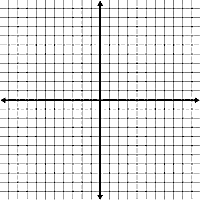
\includegraphics{graph1.png}	
    \end{center}
\part[3.5] \begin{align*}
f(x)=-(x-1)^2+2
\end{align*}
\begin{center}
	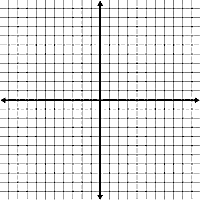
\includegraphics{graph1.png}	
\end{center}
	%\vspace{8cm}
	\part[6]  \[f(x)= \begin{cases} 
	1 & x< -2 \\
	x^2 & -2\leq x\leq 2 \\
	x &  x >2
	\end{cases}
	\]
\begin{center}
	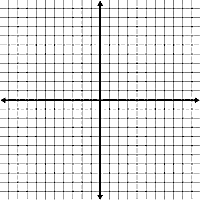
\includegraphics{graph1.png}	
\end{center}
\end{parts}

\addpoints
\question[10] Find the inverse of 
\begin{align*}
f(x)=(x-2)^3+3
\end{align*}.

\newpage
\addpoints
\question[12] Given 
\begin{align*}
f(x)=3x-2\quad \mbox{and} \quad g(x)=\frac{3}{2x-3}
\end{align*} 
then find i) $f\circ g)(x)$, ii) its domain and iii) $f\circ g)(1)$.

\vspace{8cm}
\addpoints
\question[10] A Pasture is twice as long as it is wide. Its area is $115,200 ft^2$. How wide is the pasture?

\vspace{8cm}
\newpage
\addpoints
\question[10] A Movie star, unwilling to give is age, posed the following riddle to a gossip columist: "Seven years ago, I was 11 times as old as my daughter. Now I am 4 times as old as she is." How old is the movie star?

\vspace{8cm}
\addpoints
\question[10] Find the real solution of 

\noaddpoints % If you remove this line, the grading table will show 20 points for this problem.
\begin{parts}
	\part[6] \begin{align*}
	\frac{1}{x-1}+\frac{1}{x+2}=\frac{5}{4}
	\end{align*}
	\vspace{8cm}
	\part[4]  $x^2+2x-5=0$
\end{parts}

\vspace{8cm}
\newpage
\addpoints
\question[10] Evaluate the piecewise function at the indicated values $f(-2), \quad f(1), \quad f(3)$
\begin{center}
	\[f(x)= \begin{cases} 
	x^2 & for \quad  x< 0 \\
	x+1 & for \quad x\geq 0 
	\end{cases}
	\]
\end{center}
 


\end{questions}
\end{document}